\title{ 16. Kuželosečky - parabola, hyperbola}
\author{Aneta Foralová}
\date{1.5.2025}

\maketitle

\section{Parabola, hyperbola}


\begin{figure}[H]
        \centering
        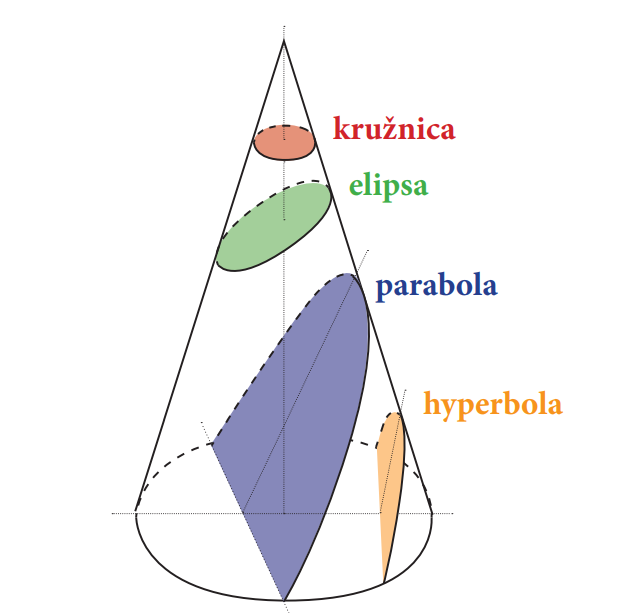
\includegraphics[width=0.3\linewidth]{img/14_kuzelosecky.png}
        \caption{Kuželosečky} 
        \label{fig:enter-label}
    \end{figure}   
    

\subsection{Definice}
    Pojem \textbf{KUŽELOSEČKY} vznikl jako název množin bodů v prostoru, které lze získat jako průniky roviny a kuželové plochy.\\
    
    Nechť je dána v rovině $E_2$ přímka $d$ a bod $F$, $F$ $\notin d$.\textbf{PARABOLA} je množina všech bodů $X$ roviny $E_2$, které mají stejnou vzdálenost od bodu $F$ i od přímky $d$\\
    
    Nechť jsou dány v rovině $E_2$ dva různé body $F$ a $G$. \textbf{HYPERBOLA} je množina všech bodů $X$ v rovině $E_2$, které mají od bodů $F$ a $G$ konstantní rozdíl vzdálenosti\\
    
    Přímka $d$ se nazývá \textbf{řídící přímka} paraboly, $V$ je \textbf{vrchol} paraboly a číslo $p$ nazýváme \textbf{parametr} a body $F$ a $G$ jsou jak u elipsy \textbf{ohniska} (U paraboly pouze 1)\\
    
    Číslo $e$ se nazývá \textbf{excentricita }hyperboly a platí $e^2=a^2 + b^2$, \textbf{Asymptoty} hyperboly jsou přímky, ke kterým se ramena hyperboly blíží, ale nikdy se jich nedotknou, určují její směr a mají tvar: $a_1: y=\frac{b/a}{a/b}x,a_2: y=-\frac{b/a}{a/b}x$
    
    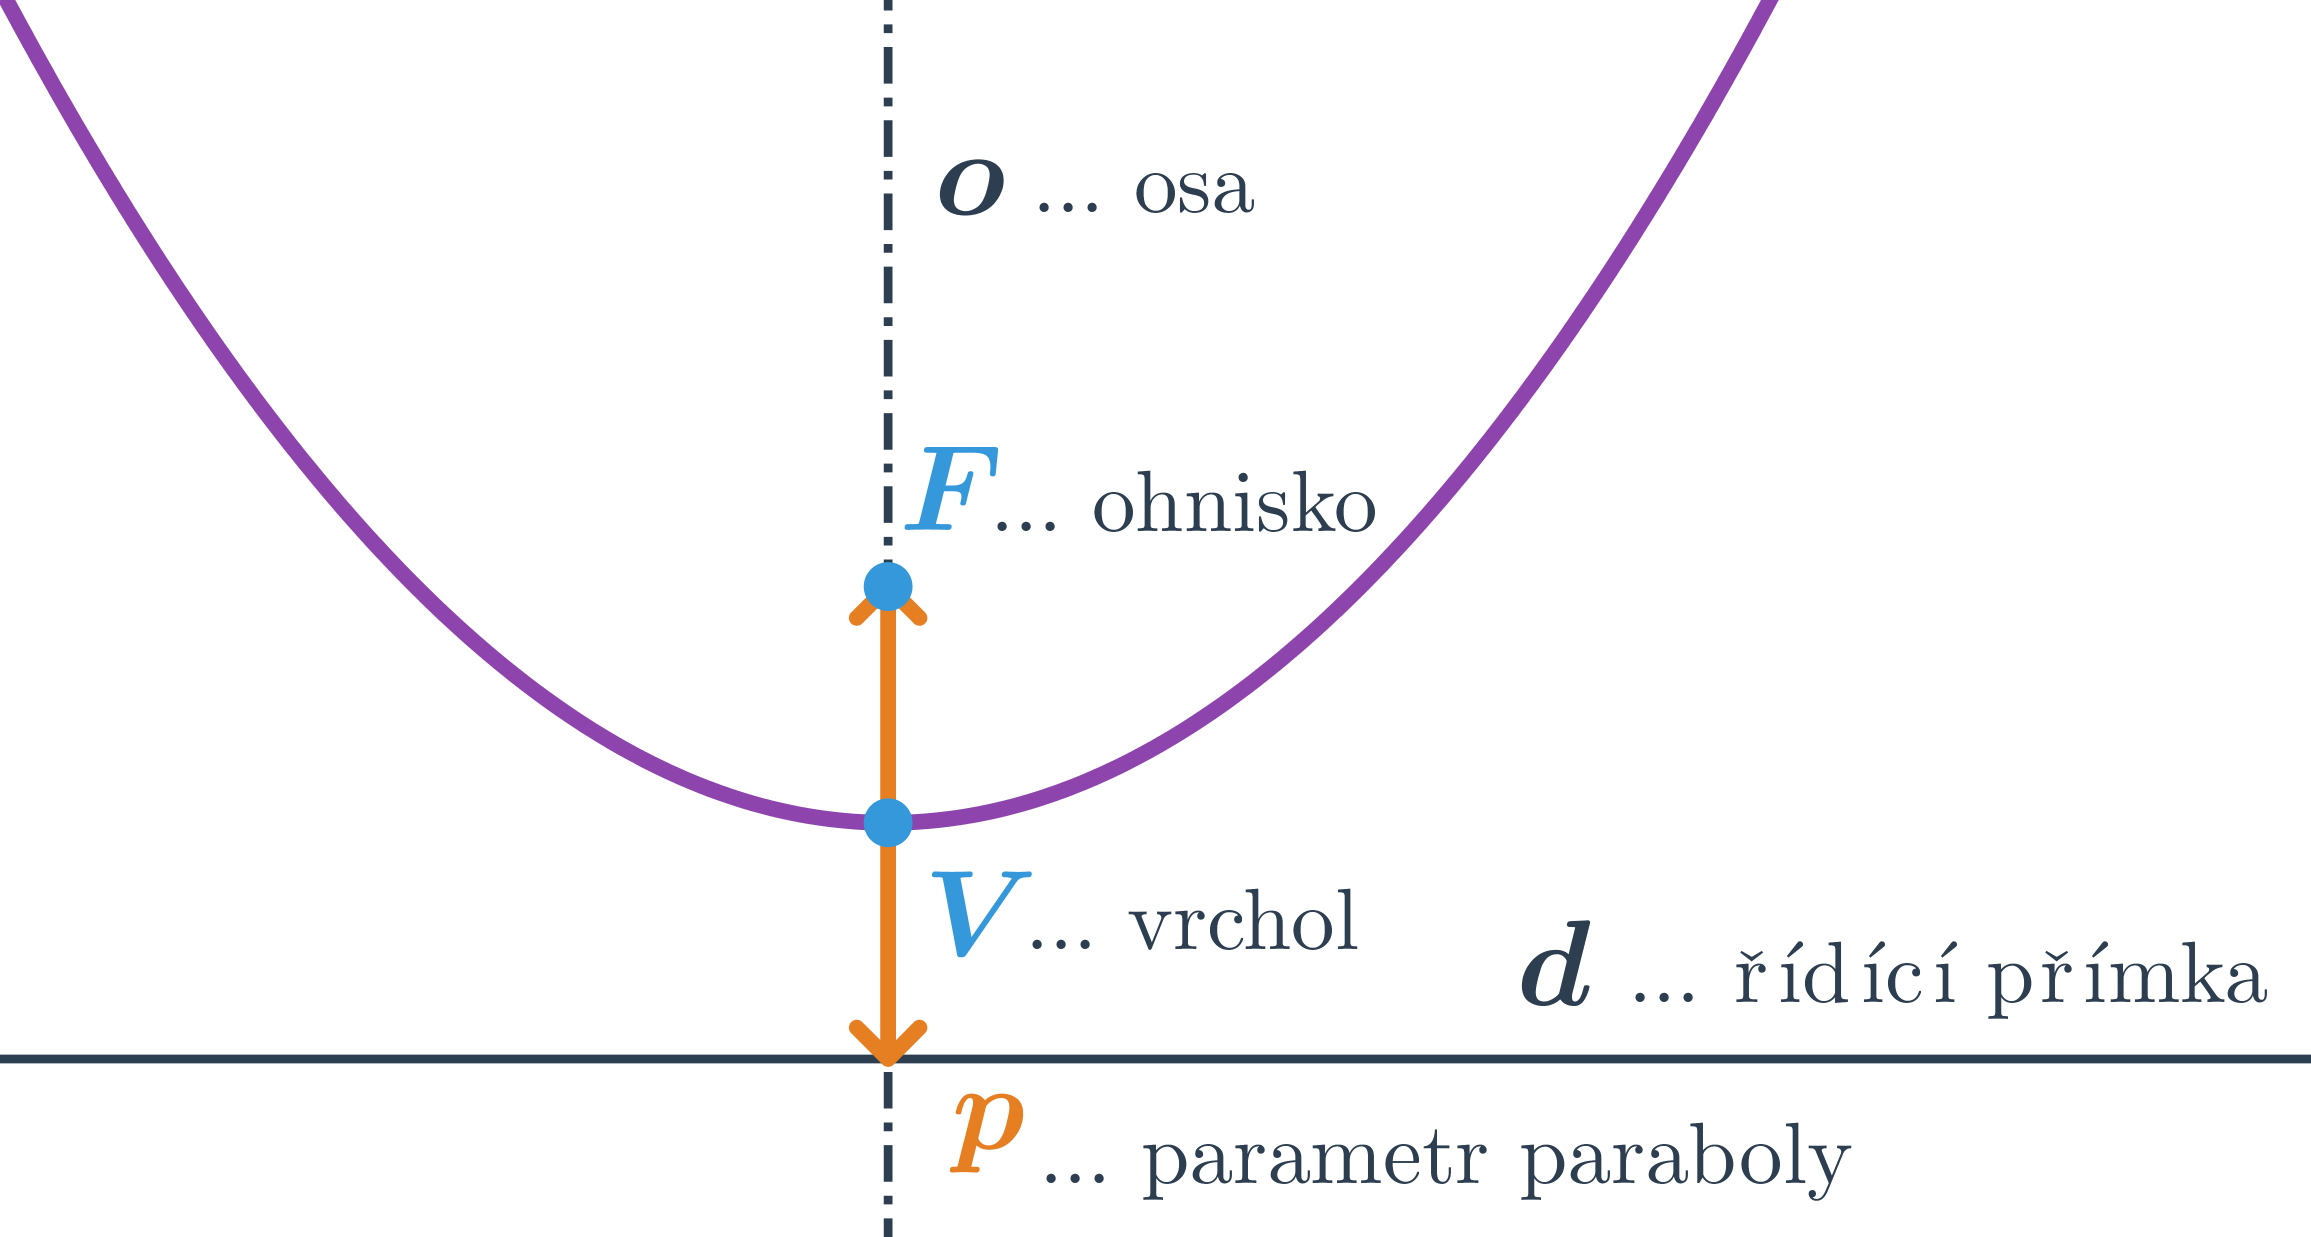
\includegraphics[width=0.45\linewidth]{img/14_parabola1.png} 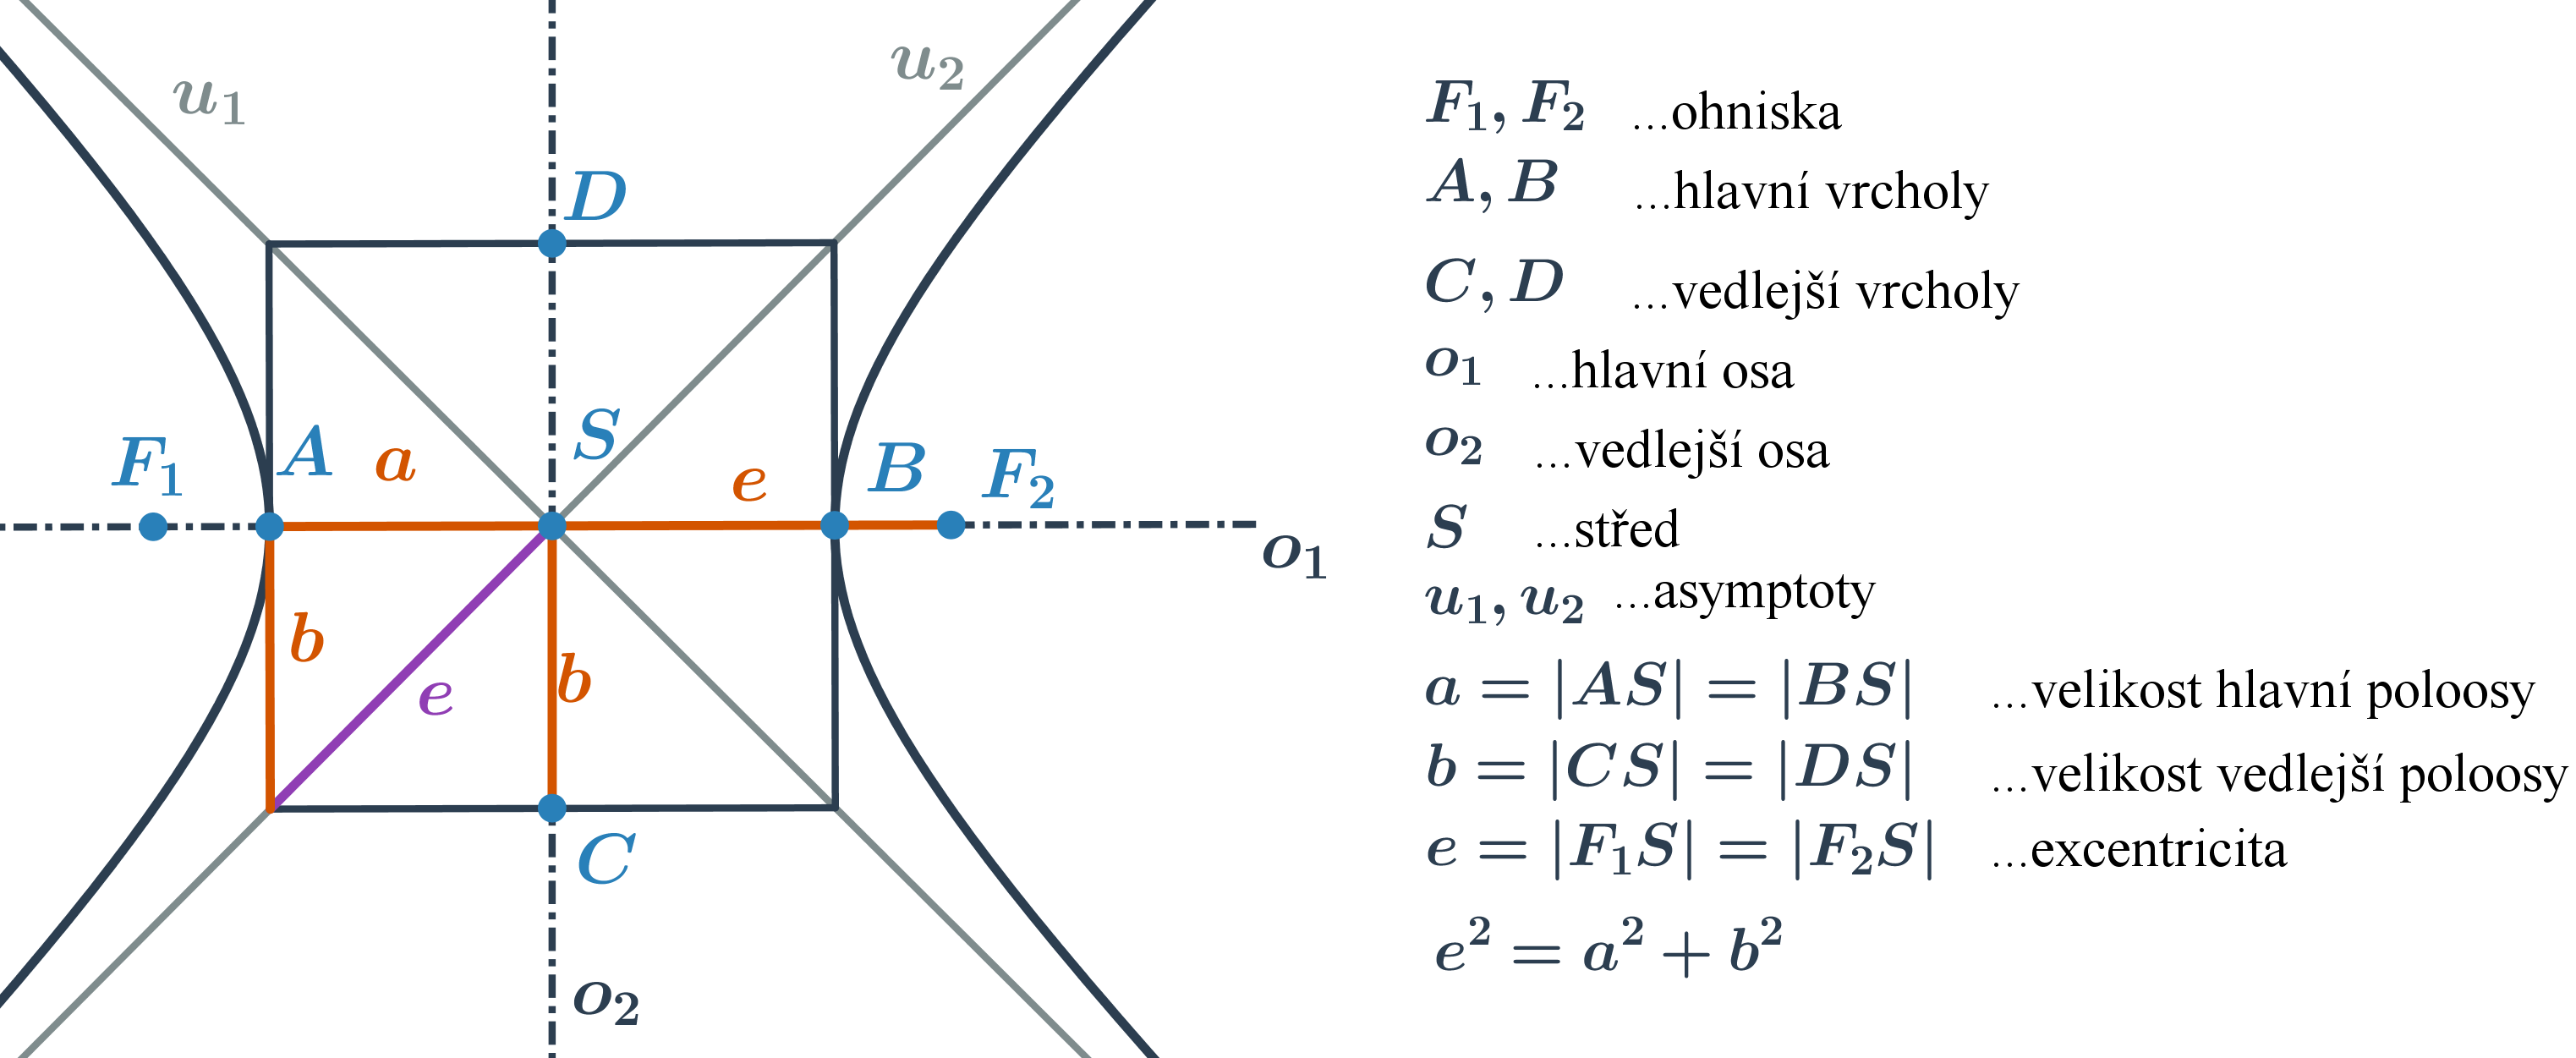
\includegraphics[width=0.7\linewidth]{img/14_hyperbola1.png}
\subsection {Středová, vrcholová a obecné rovnice}
    Obecnou rovnici kuželosečky získáme ze středové rovnice provedením operací ve středové rovnici a zavedením nových konstant\\
    Středovou rovnici kuželosečky získáme z obecné rovnice doplněním na čtverec
\subsubsection{Parabola}
    Obecná rce paraboly je: $y^2 + 2rx +2sy+t=0$ \\ 
 
    Je-li V[0;0]$2p>0$, $d= -\frac{p}{2}$ a $F[\frac{p}{2};0]$ vrcholová rovnice paraboly je: $y^2=2px$ \\
    Je-li V[0;0]$2p>0$, $d= \frac{p}{2}$ a $F[-\frac{p}{2};0]$ vrcholová rovnice paraboly je: $y^2=-2px$ \\
    Je-li V[0;0]$2p>0$, $d= -\frac{p}{2}$ a $F[0;\frac{p}{2}]$ vrcholová rovnice paraboly je: $x^2=2py$ \\
    Je-li V[0;0]$2p>0$, $d= -\frac{p}{2}$ a $F[0;-\frac{p}{2}]$ vrcholová rovnice paraboly je: $x^2=-2py$ \\

    Je-li V$[m,n]$, polopč. $VF$ a kladná poloosa x souhlasně orientované, a je omezené zleva je vrcholová rce. paraboly $(y-n)^2=2p(x-m)$\\
    Je-li V$[m,n]$, polopč. $VF$ a kladná poloosa x nesouhlasně orientované, a je omezená zprava je vrcholová rce. paraboly $(y-n)^2=-2p(x-m)$\\
    Je-li V$[m,n]$, polopč. $VF$ a kladná poloosa y souhlasně orientované, a je omezená zespoda je vrcholová rce. paraboly $(x-m)^2=2p(y-n)$\\
    Je-li V$[m,n]$, polopč. $VF$ a kladná poloosa y souhlasně orientované, a je omezená shora je vrcholová rce. paraboly $(x-m)^2=-2p(y-n)$\\
    Obecná rce paraboly je: $y^2 + 2rx +2sy+t=0$ \\
   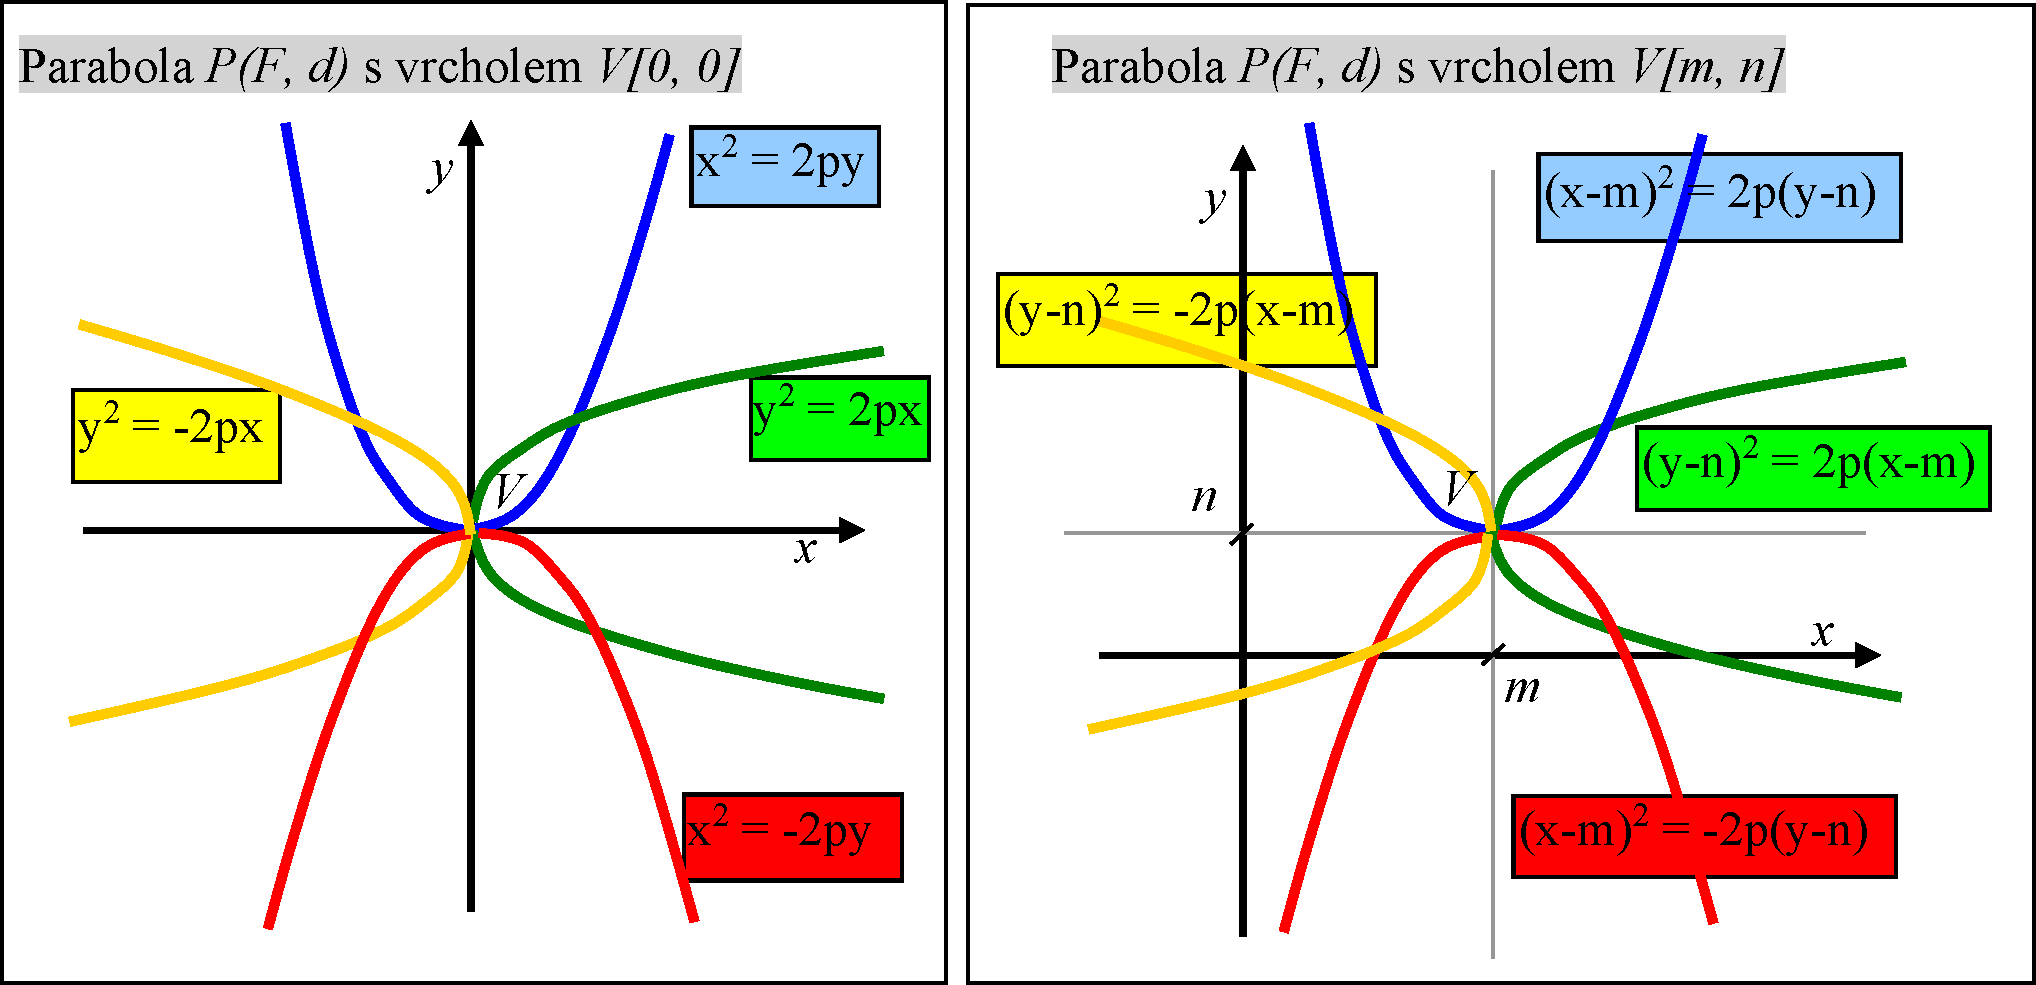
\includegraphics[width=0.8\linewidth]{img/14_parabola2.png}

\subsubsection{Hyperbola}
    Obecná rce hyperboly je: $px^2+qy^2+2rx+2sy+t=0$, kde $pq<0$ (jedno je záporné) 

    Jeli S[0;0] a hyperbola je umístěna horizontálně, je F[$-e$;0] a G[$e$;0],$a$ je hlavní poloosa a $b$ je vedlejší poloosa pak středová rovnice hyperboly je  $\frac{x^2}{a^2} - \frac{y^2}{b^2}=1$\\ 
    Jeli S[0;0] a hyperbola je umístěna vertikálně, je F[0, $e$] a G[0, $-e$] $a$ je hlavní poloosa a $b$ je vedlejší poloosa pak středová rovnice hyperboly je  $-\frac{x^2}{a^2} + \frac{y^2}{b^2}=1$\\
   
    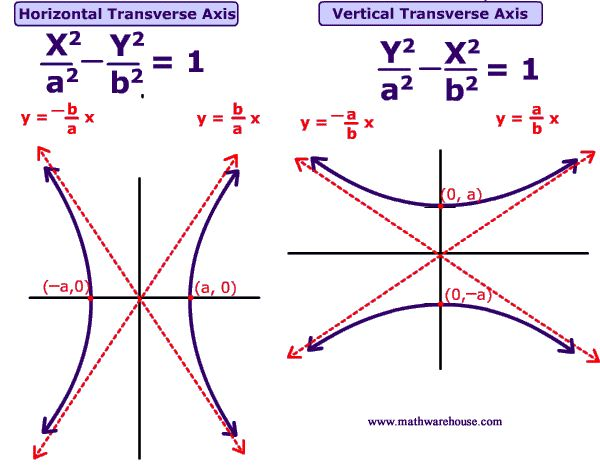
\includegraphics[width=0.5\linewidth]{img/14_hyperbola2.jpg}\\
    
    \vspace{1em}
    Je-li $S[m;n]$ a hlavní osa $o$ rovnoběžná s osou x je středová rovnice hyperboly: $\frac{(x-m)^2}{a^2} - \frac{(y-n)^2}{b^2}=1$, asymptoty mají tvar $a_1,2: (y-n)=\pm \frac{b}{a}(x-m)$
    Je-li $S[m;n]$ a hlavní osa $o$ rovnoběžná s osou y je středová rovnice hyperboly: $-\frac{(x-m)^2}{a^2} + \frac{(y-n)^2}{b^2}=1$, asymptoty mají tvar $a_1,2: (y-n)=\pm \frac{a}{b}(x-m)$
    
\subsection{Vzájemná poloha kuželosečky a bodu}
    Nechť je dána obecná rovnice kuželosečky a bod $A[x_A,y_A]$. Označíme si levou stranu obecné rovnice kuželosečky $f(x,y)$ pro každý bod kuželosečky a dosadíme souřadnice bodu $A[x_A,y_A]$ a pro jednotlivé kuželosečky platí: \begin{itemize}
        \item $A$ je bodem kuželosečky právě tehdy když $f(x_A,y_a)=0$
        \item $A$ je vnějším bodem kuželosečky právě když $f(x_A,y_a)>0$
        \item $A$ je vnitřním bodem kuželosečky právě když $f(x_A,y_a)<0$
    \end{itemize}
\subsection{Vzájemná poloha kuželosečky a přímky}
    Vzájemnou polohu kuželosečky a přímky určujeme tak, že hledáme jejich společné body. Analyticky to znamená, že hledáme řešení soustavy lineární rce (přímka) a kvadratické rce (kuželosečka) o dvou neznámých. To nakonec vede k řešení kvadratické rce o jendé neznáme. Ta může mít: \begin{itemize}
        \item Pro $D>0$ - dva společné body tj. sečna
        \item Pro $D=0$ - jedno řešení tj. tečna nebo i sečna (u paraboly, pokud přímka je rovnoběžná s osou)!
        \item Pro $D<0$ - žádné řešení tj. vnější přímka
    \end{itemize}
\subsection{Vzájemná poloha kuželoseček}
    Vzájemná poloha kuželoseček se zkoumá opět tak, že se hledají společné body, analyticky to znamená, že se řeší soustava dvou kvadratických rovnic o dvou neznámých